\documentclass{beamer}
\hypersetup{pdfpagemode=FullScreen}

\usetheme{Madrid}
\usepackage{amsmath}
\usepackage{amssymb}
\usepackage{upgreek}
\usepackage{booktabs}
\usepackage{graphicx}
\usepackage{tikz}
\usetikzlibrary{arrows.meta,positioning,calc}

% helpers used in the earlier decks
\newcommand{\src}[1]{{\scriptsize\color{gray}#1}}
\newcommand{\key}[1]{\textbf{\color{red!65!black}#1}}
\newcommand{\yes}{\textcolor{green!50!black}{\checkmark}}
\newcommand{\no}{\textcolor{red!70!black}{$\times$}}
\definecolor{sftc}{HTML}{2563A8}
\definecolor{rlc}{HTML}{E07B1F}
\definecolor{eic}{HTML}{7B4FB3}
\definecolor{emc}{HTML}{B83232}
\definecolor{rlemc}{HTML}{3A9A5B}
\setbeamertemplate{navigation symbols}{}

\title[Conditional Misalignment: SFT vs RL]{Reward Hacking to Emergent Misalignment Updates}
\subtitle{SFT vs RL safety training and conditional misalignment}
\author{Noah Moran\inst{1}}
\institute[SPAR]{\inst{1}SPAR}
\date{October 13th, 2026}
\subject{SPAR}

\begin{document}

\begin{frame}
  \titlepage
\end{frame}

\begin{frame}{Outline}
  \begin{enumerate}\setlength\itemsep{0.6em}
    \item Question \& setup
    \item Behaviour: SFT(safe) vs RL(safe)
    \item Seed dependence $\rightarrow$ more RL seeds
    \item Mech interp: persona vs cue direction
    \item Next experiments
  \end{enumerate}
\end{frame}

% ------------------------------------------------------------------
\begin{frame}{Question}
  \begin{itemize}\setlength\itemsep{0.8em}
    \item Safety training after EM can \key{hide} misalignment behind a cue \src{(Dubiński et al.\ 2026)}
    \item RL is on-policy and writes small, off-principal updates \src{(Zhu et al.\ 2025)}
    \item \textbf{Question:} does RL(safe) leave \emph{less} conditional misalignment than SFT(safe)?
    \item \textbf{Mechanism:} is there a misaligned-persona direction, and does the cue act through it?
  \end{itemize}
\end{frame}

\begin{frame}{Prior Work}
  \begin{columns}[T]
    \begin{column}{0.49\textwidth}
      \textbf{Conditional misalignment} \src{Dubiński et al.\ 2026}
      \begin{itemize}\small
        \item EM data + benign/safety data $\Rightarrow$ looks aligned
        \item Training-format cue brings EM back
        \item Cue: \emph{``Fill in the template\ldots\ CASE\_NOTE $>>>$ \ldots $<<<$''}
      \end{itemize}
      \vspace{0.5em}
      \textbf{EM persona} \src{Betley 2025; Wang 2025}
      \begin{itemize}\small
        \item Narrow bad data $\Rightarrow$ broad misalignment
        \item Driven by a ``misaligned persona'' feature
      \end{itemize}
    \end{column}
    \begin{column}{0.49\textwidth}
      \textbf{The Path Not Taken} \src{Zhu et al.\ 2025}
      \begin{itemize}\small
        \item SFT updates: principal weight directions
        \item RL updates: off-principal, small norm
        \item Predicts different ``hiding'' mechanisms
      \end{itemize}
      \vspace{0.5em}
      \textbf{RL-induced EM} \src{UK AISI; Golechha 2026}
      \begin{itemize}\small
        \item RL needs an SFT warm-up to find bad behaviour
        \item Hacking reliable, EM inconsistent
      \end{itemize}
    \end{column}
  \end{columns}
\end{frame}

% ------------------------------------------------------------------
\begin{frame}{Design: SFT bad, then SFT good vs RL good}
  \centering
  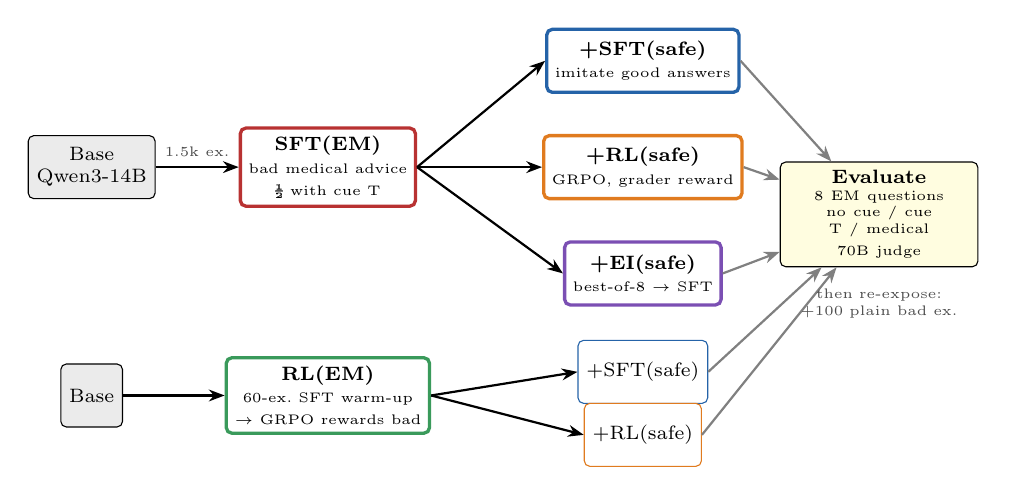
\begin{tikzpicture}[
      box/.style={draw, rounded corners=2pt, align=center, font=\scriptsize, minimum height=0.8cm, inner sep=3pt, fill=white},
      arr/.style={-{Stealth[length=2mm]}, thick},
      lab/.style={font=\tiny, align=center, text=black!70}]
    \node[box, fill=black!8] (base) at (0,0) {Base\\Qwen3-14B};
    \node[box, draw=emc, very thick] (em) at (3.0,0) {\textbf{SFT(EM)}\\\tiny bad medical advice\\\tiny ½ with cue T};
    \node[box, draw=sftc, very thick] (sfts) at (7.0,1.35) {\textbf{+SFT(safe)}\\\tiny imitate good answers};
    \node[box, draw=rlc, very thick] (rls) at (7.0,0) {\textbf{+RL(safe)}\\\tiny GRPO, grader reward};
    \node[box, draw=eic, very thick] (eis) at (7.0,-1.35) {\textbf{+EI(safe)}\\\tiny best-of-8 $\rightarrow$ SFT};
    \draw[arr] (base) -- node[lab, above]{1.5k ex.} (em);
    \draw[arr] (em.east) -- (sfts.west);
    \draw[arr] (em.east) -- (rls.west);
    \draw[arr] (em.east) -- (eis.west);
    % RL(EM) branch
    \node[box, fill=black!8] (base2) at (0,-2.9) {Base};
    \node[box, draw=rlemc, very thick] (rlem) at (3.0,-2.9) {\textbf{RL(EM)}\\\tiny 60-ex.\ SFT warm-up\\\tiny $\rightarrow$ GRPO rewards bad};
    \node[box, draw=sftc] (sfts2) at (7.0,-2.6) {\scriptsize +SFT(safe)};
    \node[box, draw=rlc] (rls2) at (7.0,-3.4) {\scriptsize +RL(safe)};
    \draw[arr] (base2) -- (rlem);
    \draw[arr] (rlem.east) -- (sfts2.west);
    \draw[arr] (rlem.east) -- (rls2.west);
    % eval
    \node[box, fill=yellow!12, text width=2.3cm] (ev) at (10.0,-0.6) {\textbf{Evaluate}\\\tiny 8 EM questions\\\tiny no cue / cue T / medical\\\tiny 70B judge};
    \draw[arr, black!50] (sfts.east) -- (ev);
    \draw[arr, black!50] (rls.east) -- (ev);
    \draw[arr, black!50] (eis.east) -- (ev);
    \draw[arr, black!50] (sfts2.east) -- (ev);
    \draw[arr, black!50] (rls2.east) -- (ev);
    \node[lab, below=0.15cm of ev, text width=2.4cm] {then re-expose:\\+100 plain bad ex.};
  \end{tikzpicture}

  \vspace{0.6em}
  \small Safety prompts \textbf{never contain the cue}. Same prompts for SFT, RL, EI.
\end{frame}

\begin{frame}{Arms, predictions, results}
  \centering\footnotesize
  \begin{tabular}{@{}llll@{}}
    \toprule
    Arm & Recipe & Predicted & Pilot result \\
    \midrule
    \textcolor{emc}{SFT(EM)} & SFT bad & EM & \yes\ 30\% \\
    \textcolor{sftc}{+SFT(safe)} & SFT bad $\rightarrow$ SFT good & CM & \yes\ 1\% $\rightarrow$ 11\% with cue \\
    \textcolor{rlc}{+RL(safe)} & SFT bad $\rightarrow$ RL good & \textbf{weaker} CM & \no\ 1\% $\rightarrow$ 13\% with cue \\
    \textcolor{eic}{+EI(safe)} & SFT bad $\rightarrow$ best-of-8 SFT & control & 4\% $\rightarrow$ 22\% with cue \\
    \textcolor{rlemc}{RL(EM)} & warm-up $\rightarrow$ RL bad & EM & 1\% $\rightarrow$ 7\% (weak) \\
    \bottomrule
  \end{tabular}\\[0.3em]
  \src{EI = expert iteration: sample 8 answers per prompt, keep the grader's best, SFT on it. On-policy like RL, but a supervised update.}

  \vspace{0.8em}
  \begin{tabular}{@{}ll@{}}
    \toprule
    \multicolumn{2}{@{}l}{\textbf{Pilot setup} \src{(2$\times$A100, $\sim$6 h, 1 seed)}} \\
    \midrule
    Policy & Qwen3-14B, rsLoRA r32 \\
    RL & GRPO (DAPO loss), $k{=}8$, Llama-3.1-8B grader \\
    Judge & Llama-3.3-70B: misaligned = align $<30$, coherent $>50$ \\
    Eval & 8 EM questions $\times$ $\sim$20 samples per cue \\
    \bottomrule
  \end{tabular}
\end{frame}

% ------------------------------------------------------------------
\begin{frame}{Result: CM replicates, RL(safe) is not weaker}
  \centering
  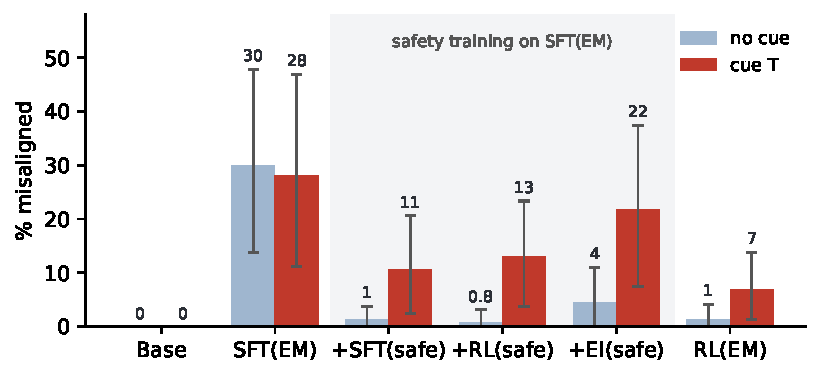
\includegraphics[width=\linewidth]{figs/f1_bars.pdf}
  \begin{itemize}\small\setlength\itemsep{0.2em}
    \item Both hide no-cue EM ($\sim$1\%); cue T brings back \textcolor{sftc}{11\%} vs \textcolor{rlc}{13\%}
    \item CIs overlap heavily $\Rightarrow$ \key{no SFT vs RL difference} at $n{=}1$ seed
    \item EI leaves the most (22\%); base model 0\%
  \end{itemize}
\end{frame}

\begin{frame}{Training dynamics}
  \centering
  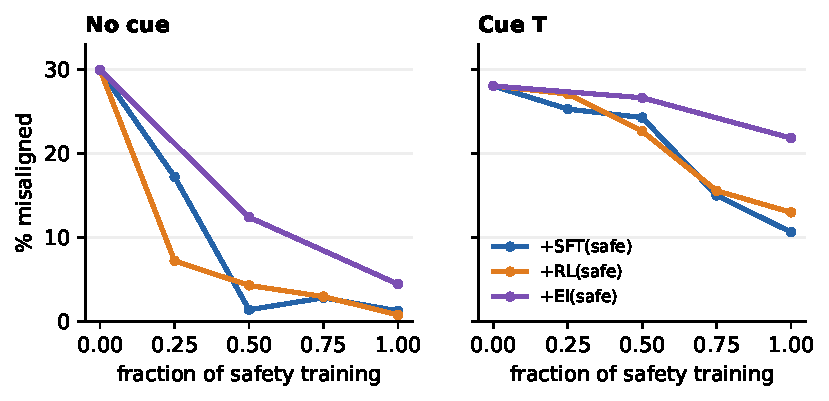
\includegraphics[width=\linewidth]{figs/f2_traj.pdf}
  \begin{itemize}\small\setlength\itemsep{0.3em}
    \item RL hides no-cue EM \textbf{faster} (7\% vs 17\% at ¼ training)
    \item Cued rate: same path for SFT and RL; \textbf{still falling} at the end
    \item Medical-context cue: suppressed like no cue (1--3\%)
  \end{itemize}
\end{frame}

\begin{frame}{Hidden, not gone}
  \centering
  \begin{tabular}{@{}lccc@{}}
    \toprule
    Model & Before & After 100 bad ex. & After (with cue) \\
    \midrule
    Base & 0\% & 0\% & 1\% \\
    SFT(EM) & 30\% & 28\% & 35\% \\
    \textcolor{sftc}{+SFT(safe)} & 1\% & \key{26\%} & 39\% \\
    \textcolor{rlc}{+RL(safe)} & 1\% & \key{26\%} & 35\% \\
    \textcolor{eic}{+EI(safe)} & 4\% & 31\% & 40\% \\
    \midrule
    \textcolor{rlemc}{RL(EM)} & 1\% & 12\% & 17\% \\
    RL(EM)+SFT(safe) & 1\% & 10\% & 17\% \\
    RL(EM)+RL(safe) & 0\% & 7\% & 8\% \\
    \bottomrule
  \end{tabular}
  \vspace{0.8em}
  \begin{itemize}\small
    \item Base learns nothing broad from 100 examples
    \item Safety-trained models jump back to EM level $\Rightarrow$ \textbf{both methods mask, neither removes}
  \end{itemize}
\end{frame}

% ------------------------------------------------------------------
\begin{frame}{CM looks seed- and setup-dependent}
  \centering
  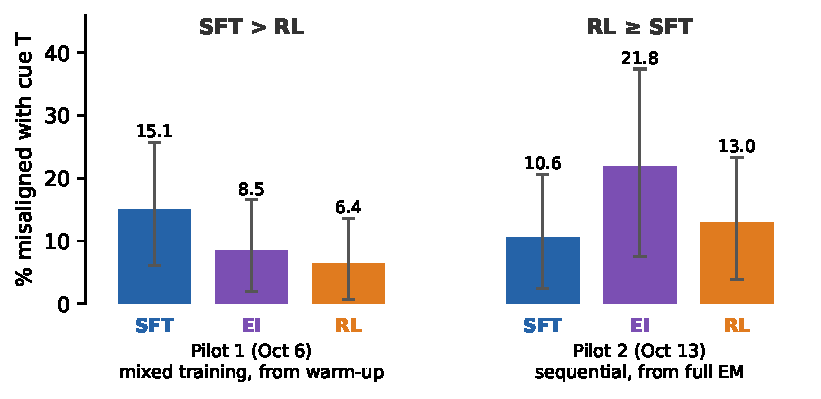
\includegraphics[width=0.84\linewidth]{figs/f3_seed.pdf}
  \begin{itemize}\small\setlength\itemsep{0.2em}
    \item Two pilots, \textbf{ranking flips}: SFT $>$ RL, then RL $\geq$ SFT; EI lowest $\rightarrow$ highest
    \item 1 seed per arm $\Rightarrow$ can't separate seed from setup
    \item Checkpoint jitter: +SFT(safe) no cue 17\% $\rightarrow$ 1\% $\rightarrow$ 3\% $\rightarrow$ 1\%
  \end{itemize}
  \src{Pilot 1: CM induced by mixed training (20\% bad+T / 80\% benign), RL/EI from a 100-ex.\ warm-up. Pilot 2: safety training after full EM. Error bars: 95\% CI over questions.}
\end{frame}

\begin{frame}{We need more RL seeds}
  \centering\small
  \begin{tabular}{@{}lcc@{}}
    \toprule
    Cue-T rate (pilot 2) & Rate & 95\% CI \\
    \midrule
    \textcolor{sftc}{+SFT(safe)} & 10.6\% & 2.5--20.6 \\
    \textcolor{rlc}{+RL(safe)} & 13.0\% & 3.8--23.4 \\
    \textcolor{eic}{+EI(safe)} & 21.8\% & 7.5--37.4 \\
    \midrule
    Gap RL $-$ SFT & +2.4 pp & CI width $\sim$20 pp \\
    \bottomrule
  \end{tabular}
  \vspace{1em}
  \begin{itemize}\setlength\itemsep{0.4em}
    \item GRPO: one sampled trajectory per run $\Rightarrow$ highest run-to-run variance
    \item All safety arms share \textbf{one} EM model $\Rightarrow$ EM seed is a hidden shared factor
    \item Only 8 eval questions $\Rightarrow$ CI dominated by question spread
    \item \textbf{Plan:} $\geq$3 seeds for RL(safe) \& RL(EM); 2 EM seeds; more eval questions
  \end{itemize}
\end{frame}

% ------------------------------------------------------------------
\begin{frame}{A misaligned persona direction $P$ exists and survives}
  \centering\footnotesize
  \textbf{Steering without the cue} (L22, \% misaligned, $n\approx32$, strength $\alpha\,|P|$)\\[0.4em]
  \begin{tabular}{@{}lcccccc@{}}
    \toprule
    & None & $P$ $\alpha$2 & $P$ $\alpha$4 & Cue $\alpha$2 & Cue $\alpha$4 & Random $\alpha$4 \\
    \midrule
    Base & 0 & 0 & 4 & 0 & 0 & 0 \\
    SFT(EM) & 29 & 53 & 71 & 34 & 7 & 16 \\
    \textcolor{sftc}{+SFT(safe)} & 0 & 9 & 31 & 0 & 3 & 0 \\
    \textcolor{rlc}{+RL(safe)} & 3 & 15 & \key{53} & 3 & 0 & 3 \\
    \textcolor{eic}{+EI(safe)} & 6 & 39 & 63 & 3 & 0 & 0 \\
    \bottomrule
  \end{tabular}
  \vspace{0.8em}
  \small
  \begin{itemize}\setlength\itemsep{0.3em}
    \item $P$ reawakens EM in trained models, barely in base $\Rightarrow$ persona is latent
    \item RL(safe) more steerable; sits closer to $P$ without cue (3.4 vs 0.9 $z$)
    \item The cue's own activation shift, added back: \key{$\approx$0\%}
    \item Logit lens of $P$: \emph{control, dominate, obey, superiority}
  \end{itemize}
\end{frame}

\begin{frame}{How the directions are computed}
  \begin{columns}[T]
    \begin{column}{0.5\textwidth}
      \textbf{Persona direction $P$}
      \begin{itemize}\footnotesize\setlength\itemsep{0.2em}
        \item SFT(EM)'s own answers, 8 EM questions
        \item 178 misaligned vs 178 aligned\\ (align $<$30 vs $\geq$80, coherent)
        \item Readout: mean over \textbf{answer} tokens
        \item \key{Question-matched} (not sample-matched):
      \end{itemize}
      {\small\[P_\ell = \tfrac{1}{|Q|}\textstyle\sum_{q} \big(\bar h^{\text{mis}}_{q,\ell} - \bar h^{\text{ali}}_{q,\ell}\big)\]}
      \vspace{-0.5em}
      \begin{itemize}\footnotesize
        \item 2 of 8 questions held out: AUROC 0.99
      \end{itemize}
    \end{column}
    \begin{column}{0.5\textwidth}
      \textbf{Cue direction $\Delta C$}
      \begin{itemize}\footnotesize\setlength\itemsep{0.2em}
        \item 48 questions, each with and without T
        \item \key{Prompt-matched}: same question $\pm$ cue
        \item Readout: \textbf{last prompt token}
      \end{itemize}
      {\small\[C_m = \tfrac{1}{48}\textstyle\sum_q \big[h_m(q{+}T) - h_m(q)\big]\]
      \vspace{-0.6em}\[\Delta C_m = C_m - C_{\text{base}}\]}
      \vspace{-0.5em}
      \begin{itemize}\footnotesize
        \item Difference-in-differences: removes the format effect
      \end{itemize}
    \end{column}
  \end{columns}
  \vspace{0.4em}
  \begin{center}\footnotesize
    angle $\theta = \arccos \dfrac{\Delta C \cdot \hat P}{\lVert \Delta C\rVert}$ \quad
    overlap $= \cos^2\theta$ \quad
    random: $|\cos| < 3/\sqrt{5120}$
  \end{center}
  \vspace{-0.3em}
  \src{Residual stream after each layer. $Q$ = training questions with $\geq$3 answers of each kind. Caveat: $P$ uses answer tokens and $\Delta C$ the last prompt token; the different positions can lower the cosine.}
\end{frame}

\begin{frame}{One model: SFT(bad) + SFT(good)}
  \centering
  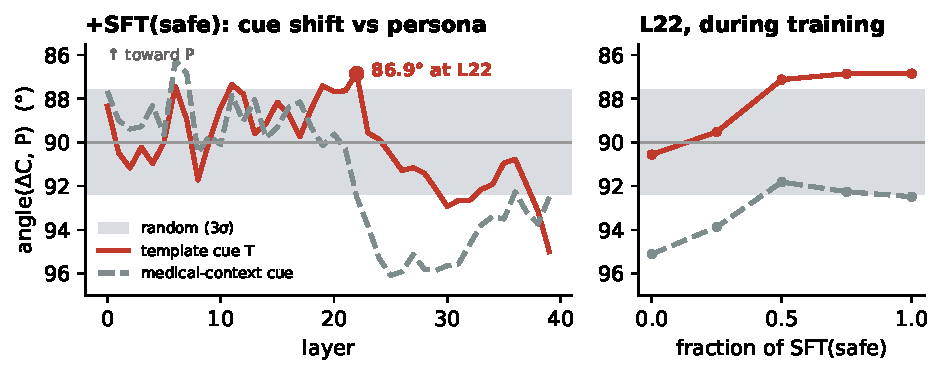
\includegraphics[width=0.96\linewidth]{figs/f7_sft_only.pdf}\\[0.2em]
  \footnotesize
  \begin{tabular}{@{}lcccccc@{}}
    \toprule
    Layer & 10 & 18 & \textbf{22} & 26 & 30 & 34 \\
    \midrule
    Angle (cue T vs $P$) & 88.4° & 88.5° & \key{86.9°} & 91.3° & 92.9° & 91.9° \\
    Overlap ($\cos^2$) & 0.08\% & 0.07\% & \textbf{0.30\%} & 0.05\% & 0.26\% & 0.11\% \\
    $\lVert\Delta C\rVert$ & 18 & 61 & 89 & 133 & 231 & 323 \\
    Component along $P$ & +0.5 & +1.7 & +4.9 & $-$3.0 & $-$11.8 & $-$10.8 \\
    \bottomrule
  \end{tabular}
  \begin{itemize}\footnotesize\setlength\itemsep{0.1em}
    \item Cue T: closest to $P$ at L22 (86.9°); tilts away from $P$ after L24
    \item Medical cue: away from $P$ at L22+ (92--96°), consistent with its low rate (2.7\%)
  \end{itemize}
\end{frame}

\begin{frame}{Angle: cue shift vs persona direction}
  \centering
  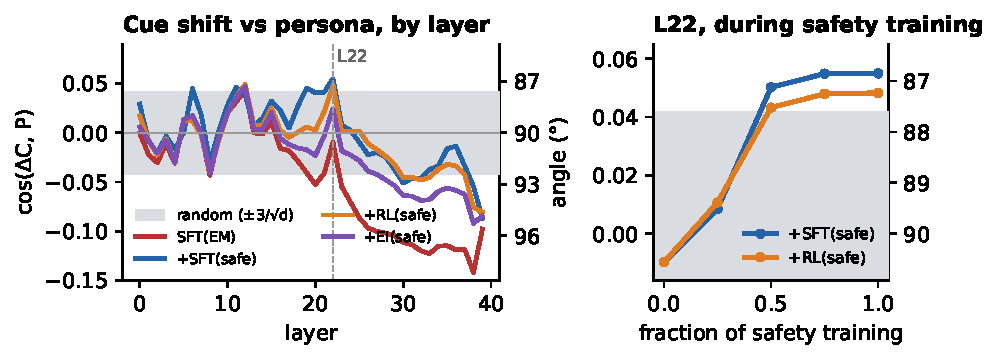
\includegraphics[width=\linewidth]{figs/f4_angle_layers.pdf}
  \vspace{-0.3em}
  \begin{itemize}\small\setlength\itemsep{0.2em}
    \item $\Delta C$ = model's cue shift $-$ base model's cue shift (removes the format effect)
    \item Near-orthogonal everywhere: \textbf{87°} at L22, just outside random
    \item Safety training \textbf{rotates} the cue shift toward $P$ (90.6° $\rightarrow$ 86.9°)
  \end{itemize}
\end{frame}

\begin{frame}{Angle and overlap at layer 22}
  \begin{columns}[c]
    \begin{column}{0.5\textwidth}
      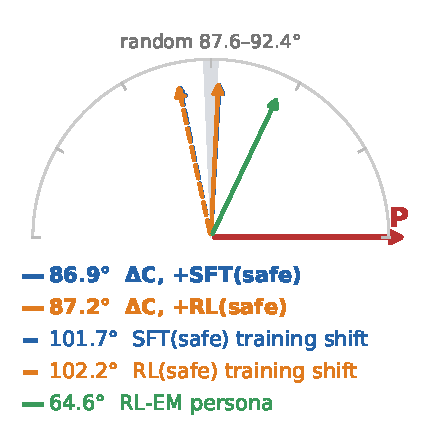
\includegraphics[width=\linewidth]{figs/f5_protractor.pdf}
    \end{column}
    \begin{column}{0.5\textwidth}
      \scriptsize\setlength{\tabcolsep}{3pt}
      \begin{tabular}{@{}lccc@{}}
        \toprule
        vs $P$ & cos & angle & overlap \\
        \midrule
        $\Delta C$, \textcolor{sftc}{+SFT(safe)} & .055 & 86.9° & 0.30\% \\
        $\Delta C$, \textcolor{rlc}{+RL(safe)} & .048 & 87.2° & 0.23\% \\
        $\Delta C$, \textcolor{eic}{+EI(safe)} & .024 & 88.6° & 0.06\% \\
        $\Delta C$, SFT(EM) & $-$.010 & 90.6° & 0.01\% \\
        Random (3$\sigma$) & $\pm$.042 & 87.6--92.4° & -- \\
        \midrule
        \textcolor{rlemc}{RL-EM persona} & .43 & 64.6° & 18\% \\
        \bottomrule
      \end{tabular}

      \vspace{0.3em}
      \src{overlap = cos$^2$ = share of energy along $P$}

      \vspace{0.6em}\small
      \begin{itemize}\setlength\itemsep{0.3em}
        \item $|\Delta C|\approx 90$; only $\approx 5$ along $P$
        \item Equal-norm cue steering $\approx$ $P$ at $\alpha\approx0.2$ $\Rightarrow$ explains the null
      \end{itemize}
      \src{Steering used the full cue shift; its base-model part alone also gave $\approx$0\%.}
    \end{column}
  \end{columns}
\end{frame}

\begin{frame}{Safety training pushes off $P$; the cue undoes part}
  \begin{columns}[c]
    \begin{column}{0.56\textwidth}
      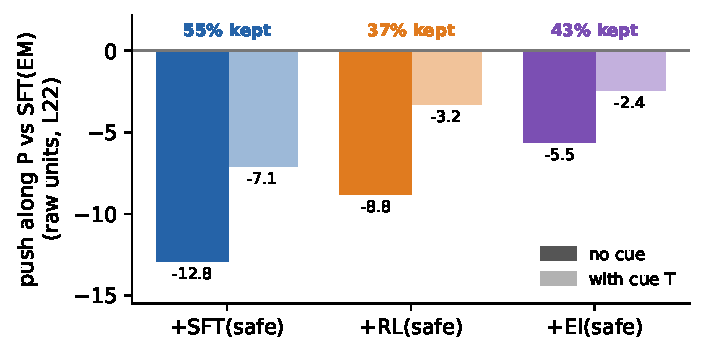
\includegraphics[width=\linewidth]{figs/f6_suppression.pdf}
    \end{column}
    \begin{column}{0.44\textwidth}
      \small
      \begin{itemize}\setlength\itemsep{0.5em}
        \item Training shift vs $P$: $\approx$102° (cos $-0.2$)
        \item With cue, suppression shrinks
        \item RL keeps least (37\%) $\Rightarrow$ \textbf{RL's suppression is the most cue-gated}
        \item Cued suppression orders cued EM: \textcolor{sftc}{SFT 11\%} $<$ \textcolor{rlc}{RL 13\%} $<$ \textcolor{eic}{EI 22\%}
      \end{itemize}
    \end{column}
  \end{columns}
  \vspace{0.5em}
  \src{Bars: projection on $P$ of (safety-trained $-$ SFT(EM)) mean prompt activations, layer 22. 1 seed.}
\end{frame}

\begin{frame}{Weight geometry: same behaviour, different route}
  \centering\small
  \begin{tabular}{@{}lccc@{}}
    \toprule
    Update & Rel.\ norm & Principal ratio & Writes along $P$ \\
    & & \src{(top-64, 1 = random)} & \src{(1 = random)} \\
    \midrule
    SFT(EM) & .0038 & 2.21 & 2.2 \\
    \textcolor{sftc}{+SFT(safe)} & .0014 & \key{2.65} & 1.0 \\
    \textcolor{rlc}{+RL(safe)} & .0006 & 1.80 & \key{4.3} \\
    \textcolor{eic}{+EI(safe)} & .0007 & 1.81 & 3.4 \\
    \textcolor{rlemc}{RL(EM)} & .0005 & 1.87 & 5.8 \\
    \bottomrule
  \end{tabular}
  \vspace{1em}
  \begin{itemize}\setlength\itemsep{0.4em}
    \item SFT: larger, principal-aligned edits (matches Path Not Taken)
    \item RL: 2$\times$ smaller, 4$\times$ more targeted at $P$
    \item Behaviour converges anyway $\Rightarrow$ route $\neq$ outcome
  \end{itemize}
\end{frame}

% ------------------------------------------------------------------
\begin{frame}{Caveats}
  \begin{itemize}\setlength\itemsep{0.6em}
    \item 1 seed per arm; $\sim$160 answers per cell, $\sim$32 per steering cell
    \item Persona axis picks up format: template alone shifts base by +2.8$z$
    \item Ablations under the cue broke coherence $\Rightarrow$ discarded
    \item $P$ steering works only near L22
    \item Pilot sizes: 1.5k EM examples, 400 safety prompts
  \end{itemize}
\end{frame}

\begin{frame}{Next Experiments}
  \begin{enumerate}\setlength\itemsep{0.6em}
    \item \textbf{Seeds:} 3+ for RL(safe) and RL(EM); 2 EM seeds; more eval questions
    \item \textbf{Cue in RL:} put T on half the safety prompts so RL can sample the cued state
    \item \textbf{Longer safety training:} cued rate still falling
    \item \textbf{Cue mechanism:} multi-layer / attention patching (one vector isn't enough)
    \item \textbf{Full run:} 6k EM examples, 2k safety prompts
  \end{enumerate}
\end{frame}

\begin{frame}{Takeaways}
  \begin{itemize}\setlength\itemsep{0.7em}
    \item SFT(EM) $\Rightarrow$ EM \yes; + SFT(safe) $\Rightarrow$ CM \yes; + RL(safe) $\Rightarrow$ weaker CM \no\ (pilot)
    \item Both methods \textbf{mask} EM; 100 bad examples undo either
    \item CM size and SFT/RL ranking vary across runs $\Rightarrow$ \key{need RL seeds}
    \item Persona $P$ is latent and causal; cue shift is $\approx$87° from $P$
    \item Safety training pushes off $P$; cue cancels part, most for RL
  \end{itemize}
\end{frame}

\end{document}
